% LREC 2022 KC Example; 
% LREC Is now using templates similar to the ACL ones. 
\documentclass[10pt, a4paper]{article}
\usepackage{lrec2022} % this is the new LREC2022 Style
\usepackage{multibib}
\newcites{languageresource}{Language Resources}
\usepackage{graphicx}
\usepackage{tabularx}
\usepackage{soul}
% for eps graphics
%%% References and Labels
%%% Reference labels without a punctuation 
% courtesy of Marc Schulder , uni Hamburg ****************
\usepackage{titlesec}
%\titleformat{\section}{\normalfont\large\bf\center}{\thesection.}{1em}{}
\titleformat{\section}{\normalfont\large\bfseries\center}{\thesection.}{1em}{}
\titleformat{\subsection}{\normalfont\SmallTitleFont\bfseries\raggedright}{\thesubsection.}{1em}{}
\titleformat{\subsubsection}{\normalfont\normalsize\bfseries\raggedright}{\thesubsubsection.}{1em}{}
\renewcommand\thesection{\arabic{section}}
\renewcommand\thesubsection{\thesection.\arabic{subsection}}
\renewcommand\thesubsubsection{\thesubsection.\arabic{subsubsection}}
%  ed 

\usepackage{epstopdf}
\usepackage[utf8]{inputenc}

\usepackage{hyperref}
\usepackage{xstring}

\usepackage{color}

\newcommand{\secref}[1]{\StrSubstitute{\getrefnumber{#1}}{.}{ }}

\title{Title of the LREC 2022 Paper (Title in 14-point Times New Roman Bold)\\ \vspace*{.5\baselineskip} \normalfont{ The Title \ul{Must Be} Capitalised as in:\\ \vspace*{.5\baselineskip} \textbf{The Rise and Fall of Ziggy Stardust and the Spiders from Mars}}}

\name{Author1, Author2, Author3} 

\address{Affiliation1, Affiliation2, Affiliation3 \\
         Address1, Address2, Address3 \\
         author1@xxx.yy, author2@zzz.edu, author3@hhh.com\\
         \{author1, author5, author9\}@abc.org\\}



\abstract{
Each paper must include an abstract of 150 to 200 words in Times New Roman 9 pt with interlinear spacing of 10 pt. The heading Abstract should be centered, font Times New Roman 10 pt bold. This short abstract will also be used for producing the Booklet of Abstracts (PDF) containing the abstracts of all papers presented at the Conference.
 \\ \newline \Keywords{keyword1, keyword2, keyword3} }

\begin{document}

\maketitleabstract

\section{Full Paper Submission}

Each full paper submission should be submitted on white A4 paper and must be between 4 and 8 pages in length (plus more pages for references if needed). 
The fully justified text should be formatted in two parallel columns. The new LREC paper dimensions are now aligned with ACL layout to ensure quick integration within the ACL Anthology. These dimensions are as follows:   
\begin{itemize}
    \item{The paper is in A4-size format, that is 21 x 29.7 cm.}
    \item{The text height is 24.7 cm and the text width 16.0 cm in two columns separated by a 0.6 cm space.}
     \item {The font for the main body of the text must be Times New Roman 10 pt with interlinear spacing of 11 pt.}
     \item {The use of LREC2022.sty will ensure the good formatting.}
 \end{itemize}

 %\color{red} check on diacritics in utf8 :  à - â - ä - é - è - ê - ë - ï - î - ô - ö - ù - û - ü - ÿ - ç %\color{black}
% ALl values have been changed KC20210901

\section{ Final Paper}

Each final paper should be submitted on white A4 paper. The fully justified text should be formatted according to LREC2022 style as indicated for the Full Paper submission.
As indicated above, the font for the main body of the text should be Times  New Roman 10 pt with interlinear spacing of 11 pt. Papers must be between 4 and 8 pages in length, including figures (plus more pages for references if needed), regardless of the mode of presentation (oral or poster).

\subsection{General Instructions for the Final Paper}
The unprotected PDF files will appear in the on-line proceedings directly as received. \textbf{Do not print the page number.}

\section{Page Numbering}

\textbf{Please do not include page numbers in your Paper.} The definitive page numbering of papers published in the proceedings will be decided by the Editorial Committee.

\section{Headings / Level 1 Headings} 

Level 1 Headings should be capitalised in the same way as the main title, and centered within the column. The font used is Times New Roman 12 pt bold. There should also be a space of 12 pt between the title and the preceding section, and a space of 3 pt between the title and the text that follows.

\subsection{Level 2 Headings}

The format of Level 2 Headings is the same as for Level 1 Headings, with the font Times New Roman 11 pt, and the heading is justified to the left of the column. There should also be a space of 6 pt between the title and the preceding section, and a space of 3 pt between the title and the text that follows.

\subsubsection{Level 3 Headings}
\label{level3H}
The format of Level 3 Headings is the same as Level 2, except that the font is Times New Roman 10 pt, and there should be no space left between the heading and the text as in \ref{level3H}. There should also be a space of 6 pt between the title and the preceding section, and a space of 3 pt between the title and the text  that follows.

%\subsubsection{Example of a sub-subsection with a long heading that will occupy two lines}
%
%Yet another example of a sub-subsection. Yet another example of a sub-subsection. Yet another example of a sub-subsection. Yet another example of a sub-subsection. Yet another example of a sub-subsection.

\section{Citing References in the Text}

\subsection{Bibliographical References}

All bibliographical references within the text should be put in between parentheses with the author's surname followed by a comma before the date of publication,\cite{Martin-90}. If the sentence already includes the author's name, then it is only necessary to put the date in parentheses: \newcite{Martin-90}. When several authors are cited, those references should be
separated with a semicolon: \cite{Martin-90,CastorPollux-92}. When the reference has more than three authors, only cite the name of the first author followed by ``et. al.'', e.g. \cite{Superman-Batman-Catwoman-Spiderman-00}.

\subsection{Language Resource References}

\subsubsection{When Citing Language Resources}
As you may know, LREC introduced a separate section on Language Resources citation to enhance the value of such assets. When citing language resources, we recommend to proceed in the same way as for bibliographical references. Please make sure to compile your Language Resources stored as a .bib file \textbf{separately} (BibTex under pdfLaTeX). This produces the required .aux et .bbl files. Thus, a language resource should be cited as \citelanguageresource{Speecon} and \citelanguageresource{EMILLE} .

\section{Figures \& Tables}
\subsection{Figures}

All figures should be centred and clearly distinguishable. They should never be drawn by hand, and the lines must be very dark in order to ensure a high-quality printed version. Figures should be numbered in the text, and have a caption in Times New Roman 10 pt underneath. A space must be left between each figure and its respective caption. 

Example of a figure enclosed in a box:

\begin{figure}[!h]
\begin{center}
%\fbox{\parbox{6cm}{
%This is a figure with a caption.}}
% old picture \includegraphics[scale=0.5]{lrec2020W-image1.eps} 
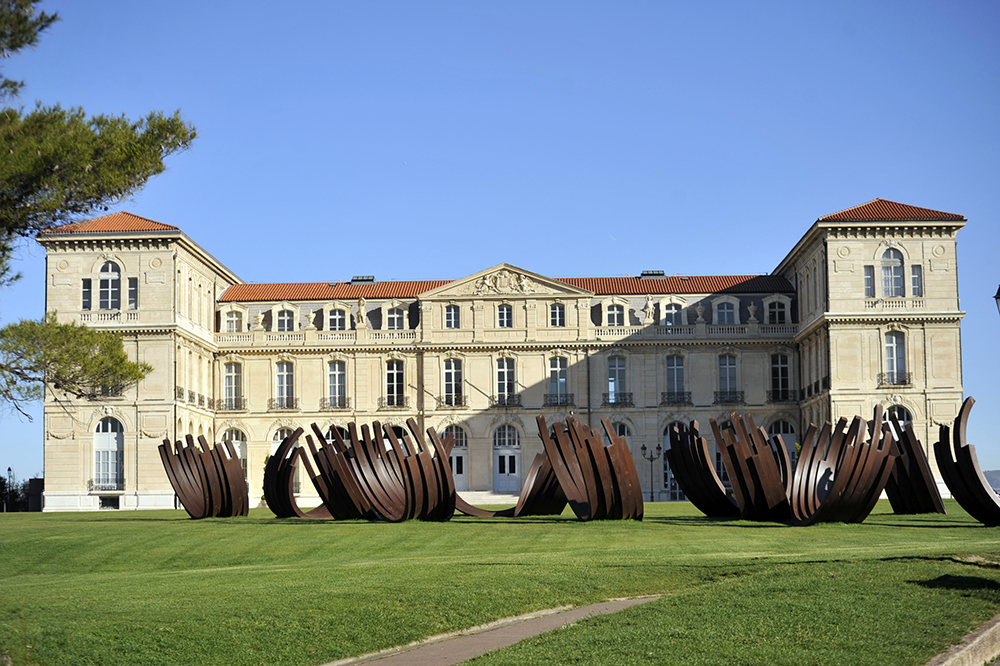
\includegraphics[scale=0.5]{pharo-marseille-3.jpg} 

\caption{The caption of the figure.}
\label{fig.1}
\end{center}
\end{figure}

Figure and caption should always appear together on the same page. Large figures can be centred, using a full page.
%NB: an example of large figures is missing.  \newpage

\subsection{Tables}

The instructions for tables are the same as for figures.
%Two types of tables are distinguished: in-column and big tables that don't fit in the columns.
%\subsection{In-column tables}
%An example of an in-column table is presented here.
%
\begin{table}[!h]
\begin{center}
\begin{tabularx}{\columnwidth}{|l|X|}

      \hline
      Level&Tools\\
      \hline
      Morphology & Pitrat Analyser\\
      \hline
      Syntax & LFG Analyser (C-Structure)\\
      \hline
     Semantics & LFG F-Structures + Sowa's\\
     & Conceptual Graphs\\
      \hline

\end{tabularx}
\caption{The caption of the table}
 \end{center}
\end{table}

%\subsection{Big tables}
%
%An example of a big table which extends beyond the column and will
%float in the next page.
%
% \begin{table*}[ht]
% \begin{center}
% \begin{tabular}{|l|l|}
%
%       \hline
%       Level&Tools\\
%       \hline\hline
%       Morphology & Pitrat Analyser\\
%       Syntax & LFG Analyser (C-Structure)\\
%       Semantics & LFG F-Structures + Sowa's Conceptual Graphs  \\
%       \hline
%
% \end{tabular}
% \caption{The caption of the big table}
% \end{center}
% \end{table*}
%

\section{Footnotes}

Footnotes are indicated within the text by a number in superscript\footnote{Footnotes should be in Times New Roman 9 pt, and appear at the bottom of the same page as their corresponding number. Footnotes should also be separated from the rest of the text by a 5 cm long horizontal line.}.

\section{Copyrights}

The Language Resouces and Evaluation Conference (LREC) Proceedings are published by the European Language Resources Association (ELRA).
They are available online from the conference website.

ELRA's policy is to acquire copyright for all LREC contributions. In assigning your copyright, you are not forfeiting your right to use your contribution elsewhere. This you may do without seeking permission and is subject only to normal acknowledgement to the LREC proceedings. The LREC 2020 Proceedings are licensed under CC-BY-NC, the Creative Commons Attribution-Non-Commercial 4.0 International License.

\section{Conclusion}

Your submission of a finalised contribution for inclusion in the LREC Proceedings automatically assigns the above-mentioned copyright to ELRA.

\section{Acknowledgements}

Place all acknowledgements (including those concerning research grants and funding) in a separate section at the end of the paper.

\section{Providing References}

\subsection{Bibliographical References} 
Bibliographical references should be listed in alphabetical order at the end of the paper. The title of the section, ``Bibliographical References'', should be a Level 1 Heading. The first line of each bibliographical reference should be justified to the left of the column, and the rest of the entry should be indented by 0.35 cm.

The examples provided in Section \ref{reference} (some of which are fictitious references) illustrate the basic format required for papers in conference proceedings, books, journal articles, PhD theses, and books chapters.

\subsection{Language Resource References}

Language resource references should be listed in alphabetical order at the end of the paper.

\section*{Appendix: How to Produce the \texttt{.pdf}}

In order to generate a PDF file out of the LaTeX file herein, when citing language resources, the following steps need to be performed:

\begin{itemize}
    \item{Compile the \texttt{.tex} file once}
    \item{Invoke \texttt{bibtex} on the eponymous \texttt{.aux} file}
 %   \item{Invoke \texttt{bibtex} on the \texttt{languageresources.aux} file}
    \item{Compile the \texttt{.tex} file twice}
\end{itemize}

% \nocite{*}
\section{Bibliographical References}\label{reference}
%\label{main:ref}

\bibliographystyle{lrec2022-bib}
\bibliography{lrec2022-example}

\section{Language Resource References}
\label{lr:ref}
\bibliographystylelanguageresource{lrec2022-bib}
\bibliographylanguageresource{languageresource}

\end{document}
